\documentclass[border = 120pt]{standalone}

\usepackage[landscape]{geometry}
\usepackage{tikz}
\usetikzlibrary{mindmap}
\usepackage{metalogo}
%\usepackage{dtklogos}
\usetikzlibrary{shapes, snakes}
\begin{document}
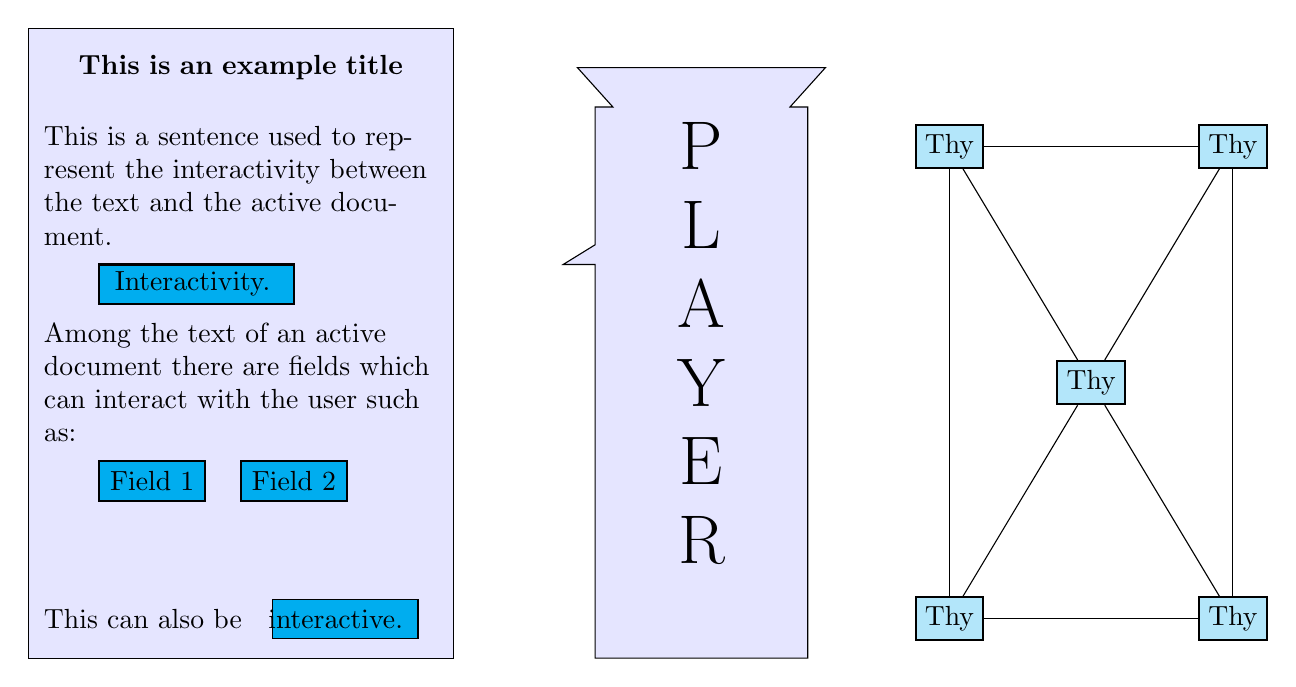
\begin{tikzpicture}[xscale=.9]

%Mother Ship
\draw[fill=blue!10] (-9,-3.5) rectangle (-15, 4.5);

%Active Document
\node[align=center, text width=5cm] at (-12,4) {\textbf{This is an example title}};
\node[align=left, text width=5cm] at (-12,2.5) {This is a sentence used to represent the interactivity between the text and the active document.};
\draw[style=thick, fill=cyan] (-14, 1.5) rectangle (-11.25, 1);
\node[align=left, text width=5cm] at (-11,1.25) {Interactivity.};

\node[align=left, text width=5cm] at (-12, 0) {Among the text of an active document there are fields which can interact with the user such as:};
\draw[style=thick, fill=cyan] (-14, -1) rectangle (-12.5, -1.5) node[pos=.5] {Field 1};
\draw[style=thick, fill=cyan] (-12, -1) rectangle (-10.5, -1.5) node[pos=.5] {Field 2};

\node[align=left, text width=5cm] at (-12,-3) {This can also be };
\draw[fill=cyan] (-11.55, -3.25) rectangle (-9.5, -2.75);
\node[align=left, text width=2cm] at (-10.5,-3) {interactive.};

% First machine
\path[draw, fill=blue!10] 
(-7, -3.5) -- 
(-7, 1.5) -- 
(-7.45, 1.5) -- 
(-7, 1.75) -- 
(-7, 3.5) -- 
(-6.75, 3.5) -- 
(-7.25, 4) -- 
(-3.75, 4) --
(-4.25, 3.5) -- 
(-4, 3.5) -- 
(-4, -3.5) -- 
cycle;

\node at (-5.5, 3) {\Huge P};
\node at (-5.5, 2) {\Huge L};
\node at (-5.5, 1) {\Huge A};
\node at (-5.5, 0) {\Huge Y};
\node at (-5.5, -1) {\Huge E};
\node at (-5.5, -2) {\Huge R};

// Nodes

\node[draw, fill=cyan!30, thick] (a) at (-2, -3) {Thy};
\node[draw, fill=cyan!30, thick] (b) at (2, -3) {Thy};
\node[draw, fill=cyan!30, thick] (c) at (2, 3) {Thy};
\node[draw, fill=cyan!30, thick] (d) at (-2, 3) {Thy};
\node[draw, fill=cyan!30, thick] (e) at (0, 0) {Thy};
\foreach \from/\to in {a/b, b/c, c/d, a/d, a/e, e/b, c/e, d/e}
\draw [-] (\from) -- (\to);

\end{tikzpicture}
\end{document}
















%%% Local Variables:
%%% mode: latex
%%% TeX-master: "report"
%%% End:
